\begin{refsection}
  
\chapter{U--Pb geochronology}\label{ch:U-Pb}

  The U--(Th--)Pb method is a rich and complex system of three
  radioactive decay chains that provide chronometric constraints on a
  wide range of geological processes, mineral phases and time scales.
  U--Pb data acquisition may focus on high throughput (using
  LA-ICP-MS), on high spatial resolution (SIMS) or on high precision
  (TIMS), and each of these analytical approaches comes with its own
  tradeofs. To accommodate this diversity in equipment and
  applications, \texttt{IsoplotR}'s U--Pb functions are more extensive
  than those of any other geochronometer. This Chapter provides an
  in-depth overview of these functions.\\

  Section~\ref{sec:UPbFormats} introduces eight different input
  formats that accommodate different types of input
  data. Section~\ref{sec:concordia} discusses three different types of
  concordia diagrams that can be used to visually assess the degree to
  which the data form a closed isotopic system, and to calculate the
  best age of such `concordant' data. Concordant data form the bedrock
  of the high precision geochronology and the geologic time scale.
  The remainder of the Chapter discusses various strategies to deal
  with discordant U--Pb compositions. Discordance can be caused by a
  range of mechanisms, such as:

  \begin{enumerate}
    \item non-radiogenic (`common') Pb.
    \item mixing of different growth zones in a texturally complex
      mineral grain.
    \item Pb-loss (or U-gain).
    \item initial disequilibrium of the \textsuperscript{235}U and
      \textsuperscript{238}U decay chains.
  \end{enumerate}

  The first three mechanisms give rise to linear (or planar) trends in
  Wetherill or Tera-Wasserburg concordia
  space. Section~\ref{sec:discordia} shows how to fit a line (or
  plane) through such data by constrained
  optimisation. Section~\ref{sec:common-Pb} shows how such isochrons
  (or `discordia') lines provides one way to correct for common Pb,
  but introduces a few other correction strategies as well.
  Section~\ref{sec:U-Pb-disequilibrium} shows how initial enrichment
  or depletion of short-lived nuclides such as \textsuperscript{234}U,
  \textsuperscript{230}Th, \textsuperscript{226}Ra or
  \textsuperscript{231}Pa can bias U--Pb ages by as much as a million
  years, and reviews some strategies to reduce this bias. Finally,
  Section~\ref{sec:discfilter} introduces methods to filter discordant
  datasets for detrital geochronology.

\section{Input formats}
\label{sec:UPbFormats}

\texttt{IsoplotR} offers eight different input formats:
\begin{enumerate}
  \item
  $\frac{07}{35}$,  
  $\mbox{err}\!\left[\frac{07}{35}\right]$, 
  $\frac{06}{38}$,  
  $\mbox{err}\!\left[\frac{06}{38}\right]$,  
  $\mbox{r}\!\left[\frac{06}{38},\frac{06}{38}\right]$
  \item $\frac{38}{06}$,  
  $\mbox{err}\!\left[\frac{38}{06}\right]$, 
  $\frac{07}{06}$,  
  $\mbox{err}\!\left[\frac{07}{06}\right]$,  
  $\left(\mbox{r}\!\left[\frac{38}{06},\frac{07}{06}\right]\right)$
  \item
  $\frac{07}{35}$,  
  $\mbox{err}\!\left[\frac{07}{35}\right]$, 
  $\frac{06}{38}$,  
  $\mbox{err}\!\left[\frac{06}{38}\right]$, 
  $\frac{07}{06}$,  
  $\mbox{err}\!\left[\frac{07}{06}\right]$, 
  $\left(\mbox{r}\!\left[\frac{07}{35},\frac{06}{38}\right]\right)$,  
  $\left(\mbox{r}\!\left[\frac{07}{35},\frac{07}{06}\right]\right)$, 
  $\left(\mbox{r}\!\left[\frac{06}{38},\frac{07}{06}\right]\right)$
  \item 
  $\frac{07}{35}$,  
  $\mbox{err}\!\left[\frac{07}{35}\right]$, 
  $\frac{06}{38}$,  
  $\mbox{err}\!\left[\frac{06}{38}\right]$,  
  $\frac{04}{38}$,  
  $\mbox{err}\!\left[\frac{04}{38}\right]$, 
  $\left(\mbox{r}\!\left[\frac{07}{35},\frac{06}{38}\right]\right)$,  
  $\left(\mbox{r}\!\left[\frac{07}{35},\frac{04}{38}\right]\right)$, 
  $\left(\mbox{r}\!\left[\frac{06}{38},\frac{04}{38}\right]\right)$
  \item 
  $\frac{38}{06}$,  
  $\mbox{err}\!\left[\frac{38}{06}\right]$, 
  $\frac{07}{06}$,  
  $\mbox{err}\!\left[\frac{07}{06}\right]$,  
  $\frac{04}{06}$,  
  $\mbox{err}\!\left[\frac{04}{06}\right]$, 
  $\left(\mbox{r}\!\left[\frac{38}{06},\frac{07}{06}\right]\right)$,  
  $\left(\mbox{r}\!\left[\frac{38}{06},\frac{04}{06}\right]\right)$, 
  $\left(\mbox{r}\!\left[\frac{07}{06},\frac{04}{06}\right]\right)$
  \item 
  $\frac{07}{35}$,  
  $\mbox{err}\!\left[\frac{07}{35}\right]$, 
  $\frac{06}{38}$,  
  $\mbox{err}\!\left[\frac{06}{38}\right]$,  
  $\frac{04}{38}$,  
  $\mbox{err}\!\left[\frac{04}{38}\right]$,  
  $\frac{07}{06}$,  
  $\mbox{err}\!\left[\frac{07}{06}\right]$, 
  $\frac{04}{07}$,  
  $\mbox{err}\!\left[\frac{04}{07}\right]$,  
  $\frac{04}{06}$,  
  $\mbox{err}\!\left[\frac{04}{06}\right]$
  \item 
  $\frac{07}{35}$,  
  $\mbox{err}\!\left[\frac{07}{35}\right]$, 
  $\frac{06}{38}$,  
  $\mbox{err}\!\left[\frac{06}{38}\right]$,  
  $\frac{08}{32}$,  
  $\mbox{err}\!\left[\frac{08}{32}\right]$,  
  $\frac{32}{38}$,  
  $\mbox{err}\!\left[\frac{32}{38}\right]$,  \\
  $\left(\mbox{r}\!\left[\frac{07}{35},\frac{06}{38}\right]\right)$,  
  $\left(\mbox{r}\!\left[\frac{07}{35},\frac{08}{32}\right]\right)$, 
  $\left(\mbox{r}\!\left[\frac{07}{35},\frac{32}{38}\right]\right)$,  
  $\left(\mbox{r}\!\left[\frac{06}{38},\frac{08}{32}\right]\right)$,  
  $\left(\mbox{r}\!\left[\frac{06}{38},\frac{32}{38}\right]\right)$, 
  $\left(\mbox{r}\!\left[\frac{08}{32},\frac{32}{38}\right]\right)$
  \item
  $\frac{38}{06}$,  
  $\mbox{err}\!\left[\frac{38}{06}\right]$, 
  $\frac{07}{06}$,  
  $\mbox{err}\!\left[\frac{07}{06}\right]$,  
  $\frac{08}{06}$,  
  $\mbox{err}\!\left[\frac{08}{06}\right]$,  
  $\frac{32}{38}$,  
  $\mbox{err}\!\left[\frac{32}{38}\right]$,  \\
  $\left(\mbox{r}\!\left[\frac{38}{06},\frac{07}{06}\right]\right)$,  
  $\left(\mbox{r}\!\left[\frac{38}{06},\frac{08}{06}\right]\right)$, 
  $\left(\mbox{r}\!\left[\frac{38}{06},\frac{32}{38}\right]\right)$,  
  $\left(\mbox{r}\!\left[\frac{07}{06},\frac{08}{06}\right]\right)$,  
  $\left(\mbox{r}\!\left[\frac{07}{06},\frac{32}{38}\right]\right)$, 
  $\left(\mbox{r}\!\left[\frac{08}{06},\frac{32}{38}\right]\right)$
\end{enumerate}

\noindent where 04, 06, 07, 08, 32, 35 and 38 stand for
\textsuperscript{204}Pb, \textsuperscript{206}Pb,
\textsuperscript{207}Pb, \textsuperscript{208}Pb,
\textsuperscript{232}Th, \textsuperscript{235}U and
\textsuperscript{238}U, respectively. `err[$\ast$]' stands for the
analytical uncertainty of $\ast$, which can be specified as a standard
error or as two times the standard error, either in absolute or
relative units. And `r[$x$,$y$]' stands for the error correlation
between $x$ and $y$.\\

Formats~1--3 are meant for mass spectrometers that are unable to
accurately measure \textsuperscript{204}Pb. This is the case for
single collector ICP-MS instruments that are unable to resolve the
isobaric interference on \textsuperscript{204}Hg, which is often
present in the plasma gas. Formats~4--6 include
\textsuperscript{204}Pb, as measured by SIMS, TIMS or multi-collector
ICP-MS. Finally, formats~7 and 8 include \textsuperscript{208}Pb and
\textsuperscript{232}Th. These nuclides can be used for hybrid
U--Th--Pb dating, as discussed in Section~\ref{sec:U-Th-Pb}.\\

Formats~1, 4 and 7 are `Wetherill style' input formats, in which the
radioactive parent appears in the denominator of the isotopic ratio
data. As explained in Section~\ref{sec:errorcorrelations} and shown in
Figure~\ref{fig:errorcorrelation}, these formats are associated with
strong error correlations
($r\left[\frac{07}{35},\frac{06}{38}\right]$), which must be specified
so as to avoid inaccurate inferences.  Formats~2, 5 and 8 are
`Tera-Wasserburg style' input formats, in which the most abundant
radiogenic daughter (i.e., \textsuperscript{206}Pb) appears in the
denominator of the isotopic ratio data.  As shown in
Figure~\ref{fig:inverrorcorrelation}, this greatly reduces the error
correlations which, consequently, are optional (hence the brackets
around $r\left[\frac{38}{06},\frac{07}{06}\right]$).\\

Finally, formats~3 and 6 provide an alternative input format designed
for users whose low level data processing software does not provide
error correlation data. It uses redundant ratios to infer the
correlation coefficients. Let $X \equiv \frac{07}{35}$, $Y \equiv
\frac{07}{35}$, $Z \equiv \frac{07}{06}$ and $U \equiv \frac{38}{35}$,
let $s[X]$, $s[Y]$ and $s[Z]$ be the standard errors of $X$, $Y$ and
$Z$, and assume that $s[U]=0$ for the sake of simplicity. Then it is
easy to see that $Z = X/(U Y)$, and
\begin{equation}
  \left(\frac{s[Z]}{Z}\right)^2 = \left(\frac{s[X/Y]}{X/Y}\right)^2
  \approx \left(\frac{s[X]}{X}\right)^2 + \left(\frac{s[Y]}{Y}\right)^2 -
  2 \frac{s[X,Y]}{XY}
  \label{eq:redundantratios}
\end{equation}

\noindent from which the covariance (and, hence, the correlation
coefficient) between $X$ and $Y$ can be inferred as
\begin{equation}
  s[X,Y] \approx \frac{XY}{2}
  \left[
    \left(\frac{s[X]}{X}\right)^2 +
    \left(\frac{s[Y]}{Y}\right)^2 -
    \left(\frac{s[Z]}{Z}\right)^2
    \right]
  \label{eq:redundantratios}
\end{equation}

It is important to note that this approach makes the crucial
assumption that all three standard errors ($s[X]$, $s[Y]$ and $s[Z]$)
are based on the same number of data points. This means that formats~3
and 6 are not applicable to TIMS data.

\section{Concordia diagrams and ages}
\label{sec:concordia}

\texttt{IsoplotR} implements three types of concordia diagram:

\begin{enumerate}
\item The \textbf{Wetherill} concordia diagram sets out the
  \textsuperscript{206}Pb/\textsuperscript{238}U vs. the
  \textsuperscript{207}Pb/\textsuperscript{235}U ratios. This format
  introduces relatively strong error correlations (see
  Section~\ref{sec:errorcorrelations}). The addition of common Pb
  pulls samples away from concordia along a line whose slope is
  proportional to the common Pb composition. Isotopic compositions
  above the concordia line are `forbidden'. They could, in principle,
  be caused by U-loss. But in practice this mechanism is implausible.
\item The \textbf{Tera-Wasserburg} concordia diagram uses the inverse
  isochron ratios \textsuperscript{207}Pb/\textsuperscript{206}Pb vs.
  and \textsuperscript{238}U/\textsuperscript{206}Pb. This format
  exhibits weaker error correlations. The addition of common Pb
  creates a binary mixing line between radiogenic and common Pb
  compositions (see Section~\ref{sec:discordia}). The area below the
  concordia line is `forbidden' and the only reason why samples may
  plot there is due to random chance and analytical imprecision.
\item The \textbf{U--Th--Pb concordia} diagram sets out the
  conventional isochron ratios of
  \textsuperscript{208}Pb/\textsuperscript{232}Th vs.
  \textsuperscript{206}Pb/\textsuperscript{238}U. Like the Wetherill
  diagram, the U--Th--Pb diagram also exhibits strong error
  correlations.  But in contrast with the Wetherill diagram, the
  addition of common Pb does not necessarily create linear trends on
  the U--Th--Pb diagram. Instead, different aliquots may end up on
  either side of the concordia line depending on their Th/U ratio.
\end{enumerate}

The Wetherill and Tera-Wasserburg concordia plots are available to
datasets from any of \texttt{IsoplotR}'s eight input formats,
irrespective of whether the ratios are stored in a Wetherill or
Tera-Wasserburg format. \texttt{IsoplotR} automatically handles the
data conversions internally. The U--Th--Pb concordia plot is only
available for data formats~7 and 8, because these are the only formats
that account for \textsuperscript{208}Pb and \textsuperscript{232}Th.
The remainder of this Chapter will focus on the Wetherill and
Tera-Wasserburg diagrams, except for Section~\ref{sec:common-Pb},
which will briefly mention the U--Th-Pb diagram again.\\

\noindent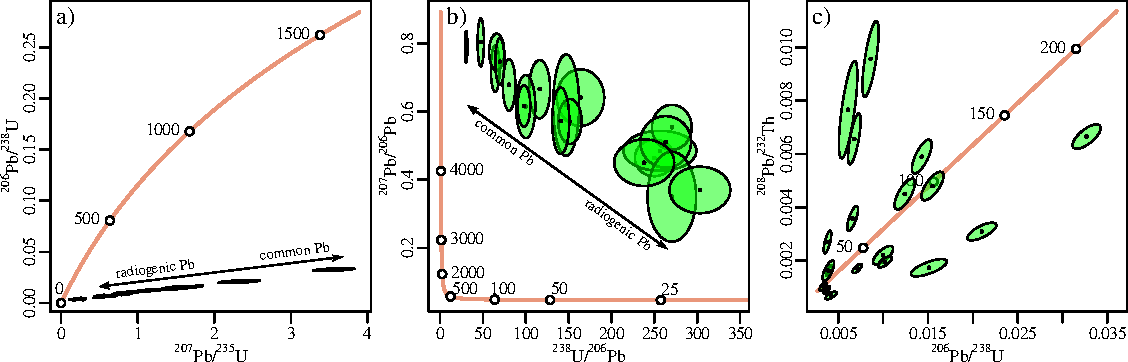
\includegraphics[width=\textwidth]{../figures/3xconcordia.pdf}
\begingroup \captionof{figure}{The allanite dataset of
  \citet{janots2014} shown on a) Wetherill, b) Tera-Wasserburg and c)
  U--Th--Pb concordia diagrams.\\}\endgroup

In the absence of (or after correction for) common Pb or other
complications, multiple aliquots from the same sample may plot on the
concordia line. Such samples are said to be concordant. Their `most
likely' age (in a statistical sense) is known as the \textbf{concordia
  age}. Calculating a concordia age involves two steps
\citep{ludwig1998}:

\begin{enumerate}
  \item Calculate the two-dimensional error-weighted average
    ($\{\bar{x},\bar{y}\}$) of the U--Pb ratios, by minimising the sum
    of squares $S$ or, equivalently, by maximising the likelihood for
    equivalence 
    $\mathcal{LL}_e$. In Wetherill space:
    \begin{equation}
      \mathcal{LL}_e \propto - \frac{S_e}{2} =
      -\frac{1}{2}\sum\limits_{i=1}^{n} \left[
      \begin{array}{@{}c@{}}
        \left[\frac{07}{35}\right]_i-\bar{x}\\
        \left[\frac{06}{38}\right]_i-\bar{y}
      \end{array}
      \right]^T
    \left[
      \begin{array}{@{}cc@{}}
        s\!\left[\frac{07}{35}\right]_i^2 &
        s\!\left[\frac{07}{35},\frac{06}{38}\right]_i\\
        s\!\left[\frac{07}{35},\frac{06}{38}\right]_i &
        s\!\left[\frac{06}{38}\right]_i^2
      \end{array}
      \right]^{-1}
    \left[
      \begin{array}{@{}c@{}}
        \left[\frac{07}{35}\right]_i-\bar{x}\\
        \left[\frac{06}{38}\right]_i-\bar{y}
      \end{array}
      \right]    
    \end{equation}

    or in Tera-Wasserburg space:
        \begin{equation}
    \mathcal{LL}_e \propto - \frac{S_e}{2} =
      -\frac{1}{2}\sum\limits_{i=1}^{n}
    \left[
      \begin{array}{@{}c@{}}
        \left[\frac{38}{06}\right]_i-\bar{x}\\
        \left[\frac{07}{06}\right]_i-\bar{y}
      \end{array}
      \right]^T
    \left[
      \begin{array}{@{}cc@{}}
        s\!\left[\frac{38}{06}\right]_i^2 &
        s\!\left[\frac{38}{06},\frac{07}{06}\right]_i\\
        s\!\left[\frac{38}{06},\frac{07}{06}\right]_i &
        s\!\left[\frac{07}{06}\right]_i^2
      \end{array}
      \right]^{-1}
    \left[
      \begin{array}{@{}c@{}}
        \left[\frac{38}{06}\right]_i-\bar{x}\\
        \left[\frac{07}{06}\right]_i-\bar{y}
      \end{array}
      \right]    
    \end{equation}

    Using standard maximum likelihood theory, the covariance matrix of
    the weighted mean composition ($\Sigma_{\bar{x},\bar{y}}$) is
    obtained by inverting the Fisher information matrix.
    
  \item Given the concordia composition $\{\bar{x},\bar{y}\}$ obtained
    in the previous step, compute the most likely age ($t_c$) of this
    concordia composition. This is done by maximising the likelihood
    of concordance. In Wetherill space:
        \begin{equation}
    \mathcal{LL}_c \propto - \frac{S_c}{2} =
      -\frac{1}{2}\sum\limits_{i=1}^{n}
    \left[
      \begin{array}{@{}c@{}}
        \bar{x} - (\exp[\lambda_{235}t_c] - 1)\\
        \bar{y} - (\exp[\lambda_{238}t_c] - 1)
      \end{array}
      \right]^T
    \Sigma_{\bar{x},\bar{y}}^{-1}
    \left[
      \begin{array}{@{}c@{}}
        \bar{x} - (\exp[\lambda_{235}t_c] - 1)\\
        \bar{y} - (\exp[\lambda_{238}t_c] - 1)
      \end{array}
      \right]
    \label{eq:concordiaAgeWetherill}
    \end{equation}

    Or in Tera-Wasserburg space:
        \begin{equation}
    \mathcal{LL}_c \propto - \frac{S_c}{2} =
      -\frac{1}{2}\sum\limits_{i=1}^{n}
    \left[
      \begin{array}{@{}c@{}}
        \bar{x} - \frac{1}{\exp[\lambda_{238}t_c] - 1}\\
        \bar{y} - \left[\frac{35}{38}\right]
        \frac{\exp[\lambda_{235}t_c] - 1}
             {\exp[\lambda_{238}t_c] - 1}
      \end{array}
      \right]^T
    \Sigma_{\bar{x},\bar{y}}^{-1}
    \left[
      \begin{array}{@{}c@{}}
        \bar{x} - \frac{1}{\exp[\lambda_{238}t_c] - 1}\\
        \bar{y} - \left[\frac{35}{38}\right]
        \frac{\exp[\lambda_{235}t_c] - 1}
             {\exp[\lambda_{238}t_c] - 1}
      \end{array}
      \right]
    \label{eq:concordiaAgeTW}
    \end{equation}

    Again, the uncertainty of $t_c$ is obtained from the Fisher
    information matrix.
    
\end{enumerate}

The same concordia age is obtained regardless of whether the
calculations are carried out in Wetherill or Tera-Wasserburg space.\\

\noindent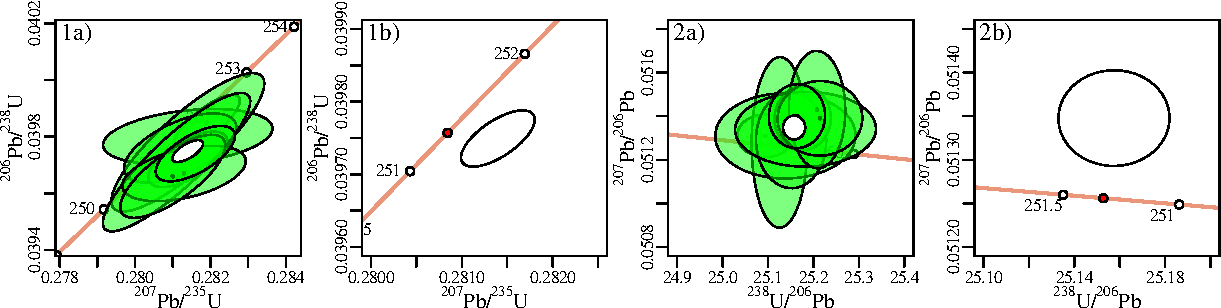
\includegraphics[width=\textwidth]{../figures/concordia_age.pdf}
\begingroup \captionof{figure}{1) Wetherill and 2) Tera-Wasserburg
  concordia diagram with a) the weighted mean composition shown as
  white error ellipse, and b) the concordia age (251.3~Ma) is shown as
  a red circle.\\}\endgroup

The goodness-of-fit can be quantified either using a chi-square test,
or with the MSWD. We can define three p-values and three MSWD values:

\begin{description}
\item{concordance}: MSWD\textsubscript{c} $= S_c$
\item{equivalence}: MSWD\textsubscript{e} $= S_e/(2n-2)$
\item{combined}: MSWD $= (S_e + S_c)/(2n-1)$
\end{description}

\noindent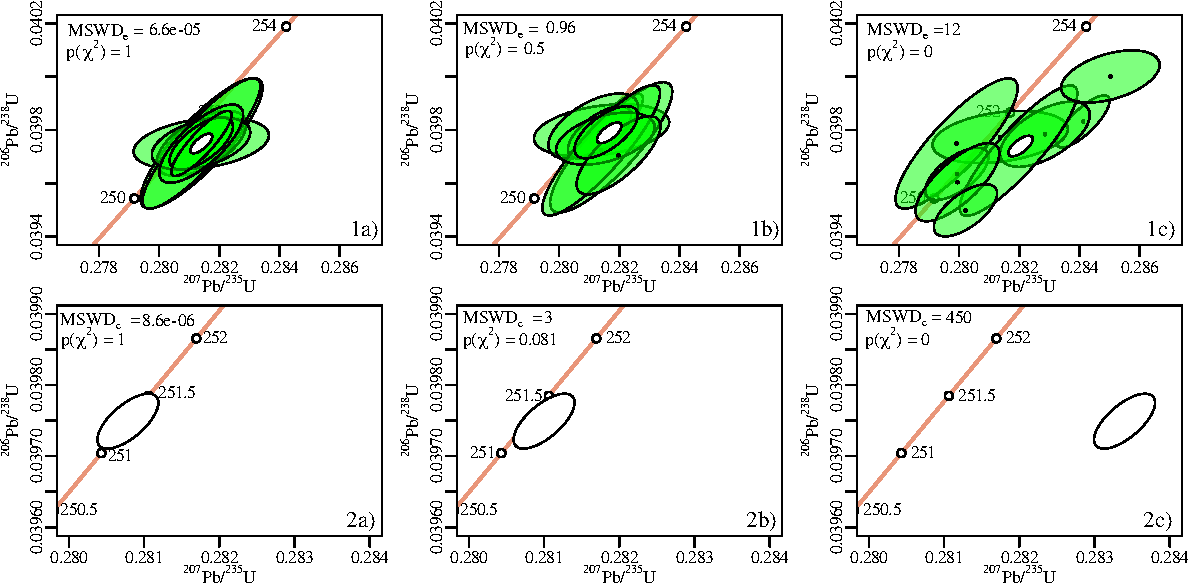
\includegraphics[width=\textwidth]{../figures/concordia_MSWD.pdf}
\begingroup \captionof{figure}{MSWDs and p-values for 1) equivalence
  and 2) concordance for data that are a) underdispersed, b) dispersed
  by an amount that is consistent with the analytical uncertainties,
  and c) overdispersed with respect to the analytical
  uncertainties.\\}\endgroup

In high precision geochronology, the analytical uncertainty of the
uranium decay constants becomes a significant factor in assessing the
degree of concordance. This uncertainty represents a systematic error,
which can be added to the covariance matrix of the weighted mean
composition:
\begin{equation}
  \Sigma_{\bar{x},\bar{y}}^{'} =
  \Sigma_{\bar{x},\bar{y}} + t_c^2
  \left[
    \begin{array}{@{}c@{}}
      \exp[\lambda_{235}t_c] \\
      \exp[\lambda_{238}t_c]      
    \end{array}
    \right]^T
  \left[
    \begin{array}{@{}cc@{}}
      \sigma[\lambda_{235}]^2 & \sigma[\lambda_{235},\lambda_{238}] \\
      \sigma[\lambda_{235},\lambda_{238}] & \sigma[\lambda_{238}]^2
    \end{array}
    \right]
  \left[
    \begin{array}{@{}c@{}}
      \exp[\lambda_{235}t_c]\\
      \exp[\lambda_{238}t_c]
    \end{array}
    \right]
  \label{eq:systematicUPb}
\end{equation}

\noindent where $\sigma[\lambda_{235}]$, $\sigma[\lambda_{238}]$ and
$\sigma[\lambda_{235},\lambda_{238}]$ are the (co)variances of the
\textsuperscript{235}U and \textsuperscript{238}U decay constants.
\texttt{IsoplotR} visualises the decay constant uncertainties by
increasing the width of the concordia line, and takes them into
account when calculating the MSWD and p-value of concordance:

\begin{center}
\noindent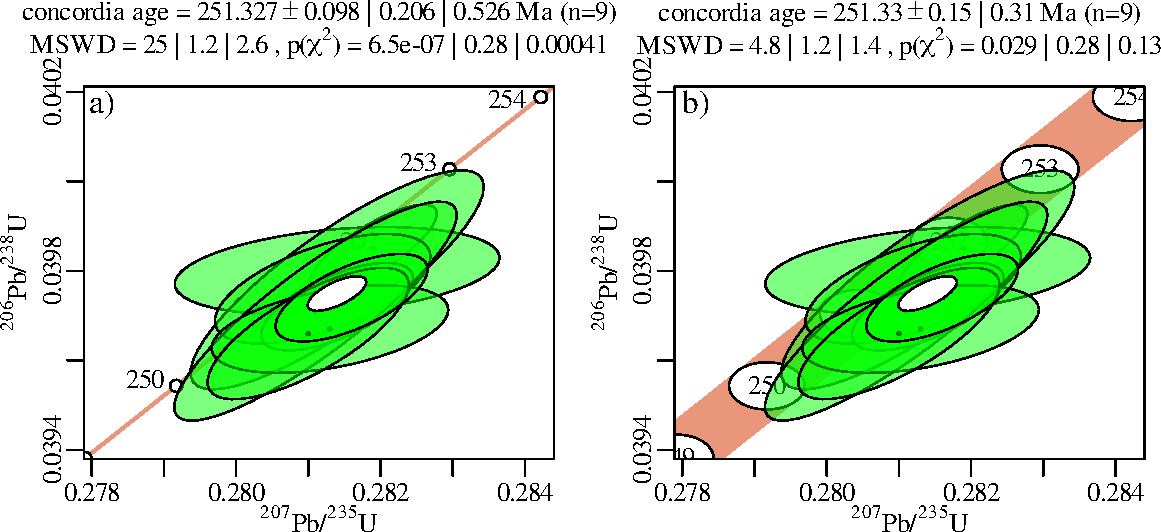
\includegraphics[width=.85\textwidth]{../figures/concexterr.pdf}
\captionof{figure}{Wetherill concordia diagram with concordia age
  calculations a) without and b) with decay constant uncertainties.
  The legends report the MSWD and p-value for concordance $\mid$
  equivalence $\mid$ concordance + equivalence. Taking into account
  the decay constant uncertainty decreases the value of
  MSWD\textsubscript{c} and increases the p-value of concordance.}
\end{center}

\section{Discordia/isochron regression}
\label{sec:discordia}

As discussed in the introductory paragraphs of this Chapter, U--Pb
data can form linear trends in Wetherill or Tera-Wasserburg concordia
space due to:

\begin{enumerate}
\item the addition of non-radiogenic Pb components (`common Pb');
\item binary mixing of different aged growth zones;
\item partial loss of radiogenic Pb.
\end{enumerate}

\texttt{IsoplotR} uses three different algorithms to fit these linear
trends:

\begin{enumerate}
\item formats 1--3: Semitotal-U/Pb regression using
  \textsuperscript{206/7}Pb and \textsuperscript{238}U. Let
  $\left[\frac{07}{06}\right]_i$ and $\left[\frac{38}{06}\right]_i$ be
  $n$ \textsuperscript{207}Pb/\textsuperscript{206}Pb and
  \textsuperscript{238}U/\textsuperscript{206}Pb ratio
  measurements\footnote{the same calculation can also be carried out
    in Wetherill space but is omitted here for brevity.},
  respectively. Then this algorithm chooses the common Pb composition
  $\left[\frac{07}{06}\right]_\circ$ and concordia intercept age $t$
  that best fits the following mixing line in a maximum likelihood
  sense:
  \begin{equation}
    \left[\frac{07}{06}\right]_i = \left[\frac{07}{06}\right]_\circ -
    \left[\frac{38}{06}\right]_i\left\{
    \left[\frac{07}{06}\right]_\circ\left(\exp[\lambda_{238}t]-1\right)
    -\left[\frac{35}{38}\right]_i\left(\exp[\lambda_{235}t]-1\right)
    \right\}
    \label{eq:semitotal-U/Pb}
  \end{equation}

  \noindent\begin{minipage}[t]{.3\linewidth}
  \strut\vspace*{-\baselineskip}\newline
  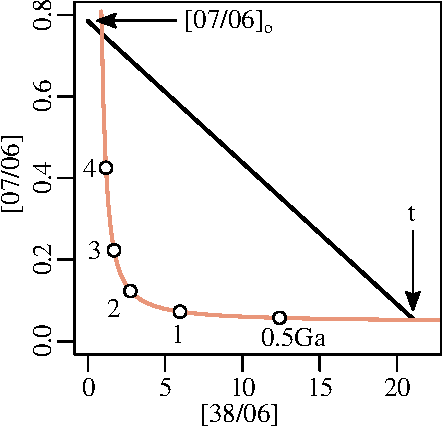
\includegraphics[width=\textwidth]{../figures/UPbisochron13.pdf}
  \end{minipage}
  \begin{minipage}[t]{.7\linewidth}
    \captionof{figure}{The semitotal-U/Pb isochron is a binary mixture
      line between a non-radiogenic Pb component with
      \textsuperscript{207}Pb/\textsuperscript{206}Pb ratio
      $[07/06]_\circ$ and a radiogenic
      \textsuperscript{238}U/\textsuperscript{206}Pb ratio that marks
      a point on the concordia line corresponding to an age $t$.}
    \label{fig:UPbisochron13}
  \end{minipage}

\item\label{it:UPbIsochron46} formats 4--6: Total-U/Pb regression
  using \textsuperscript{204/6/7}Pb and \textsuperscript{235/8}U
  \citep{ludwig1998}.  Given $n$ sets of three-dimensional isotopic
  ratio measurements this algorithm can be formulated as a system of
  two equations that describe two coupled mixing lines with two common
  Pb intercepts ($\left[\frac{04}{06}\right]_\circ$ and
  $\left[\frac{04}{07}\right]_\circ$) and a single concordia intercept
  age $t$:
    \begin{align}
    \left[\frac{04}{06}\right]_i & =
    \left[\frac{04}{06}\right]_\circ
    \left\{
    1 - \left[\frac{38}{06}\right]_i(\exp[\lambda_{238}t]-1)
    \right\} \label{eq:total-U/Pb-a} \\
    \left[\frac{04}{07}\right]_i & =
    \left[\frac{04}{07}\right]_\circ
    \left\{
    1 - \left[\frac{35}{07}\right]_i(\exp[\lambda_{235}t]-1)
    \right\}
    \label{eq:total-U/Pb-b}
    \end{align}
    
  \noindent\begin{minipage}[t]{.6\linewidth}
  \strut\vspace*{-\baselineskip}\newline
  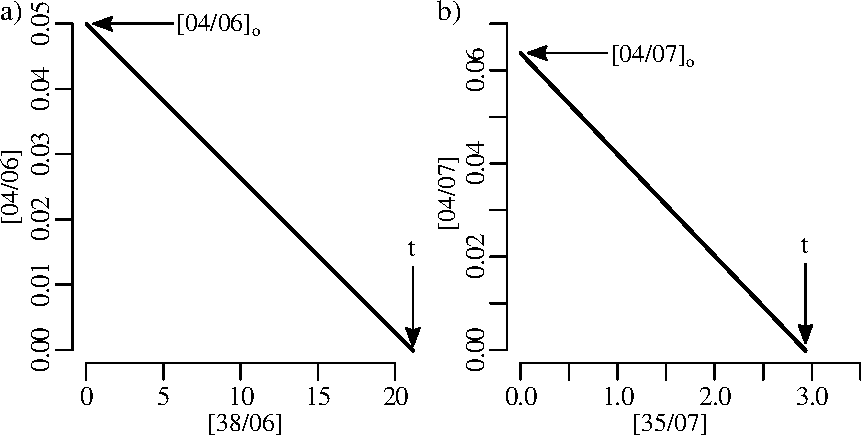
\includegraphics[width=\textwidth]{../figures/UPbisochron46.pdf}
  \end{minipage}
  \begin{minipage}[t]{.4\linewidth}
    \captionof{figure}{The total-U/Pb isochron is a binary mixture
      line between a non-radiogenic Pb component with
      \textsuperscript{204}Pb/\textsuperscript{206}Pb and
      \textsuperscript{204}Pb/\textsuperscript{207}Pb ratios
      $[04/06]_\circ$ and $[04/07]_\circ$, and radiogenic
      \textsuperscript{238}U/\textsuperscript{206}Pb and
      \textsuperscript{235}U/\textsuperscript{207}Pb ratios that mark
      a point on the concordia line corresponding to an age $t$.  a)
      shows Equation~\ref{eq:total-U/Pb-a}, b) shows
      Equation~\ref{eq:total-U/Pb-b}.}
    \label{fig:UPbisochron46}
  \end{minipage}

\item\label{it:UPbIsochron78} formats 7 and 8: Total-U-Th/Pb
  regression using \textsuperscript{206/7/8}Pb \textsuperscript{232}Th
  and \textsuperscript{235/8}U \citep{vermeesch2021}. If
  \textsuperscript{204}Pb cannot be measured precisely enough, then we
  can use \textsuperscript{208}Pb as a proxy for common Pb, after
  correction for the radiogenic contribution from
  \textsuperscript{232}Th:
    \begin{align}
      \left[\frac{08}{06}\right]_i -
      \left[\frac{32}{38}\right]_i
      \left[\frac{38}{06}\right]_i
      \left(\exp[\lambda_{232}t]-1\right)
      & =
    \left[\frac{08}{06}\right]_\circ
    \left\{
    1 - \left[\frac{38}{06}\right]_i(\exp[\lambda_{238}t]-1)
    \right\} \label{eq:total-U-Th/Pb-a} \\
      \left[\frac{08}{07}\right]_i -
      \left[\frac{32}{38}\right]_i
      \left[\frac{38}{35}\right]
      \left[\frac{35}{07}\right]_i
      \left(\exp[\lambda_{232}t]-1\right)
      & =
    \left[\frac{08}{07}\right]_\circ
    \left\{
    1 - \left[\frac{35}{07}\right]_i(\exp[\lambda_{235}t]-1)
    \right\}
    \label{eq:total-U-Th/Pb-b}
    \end{align}

    \noindent\begin{minipage}[t][][b]{\linewidth}
    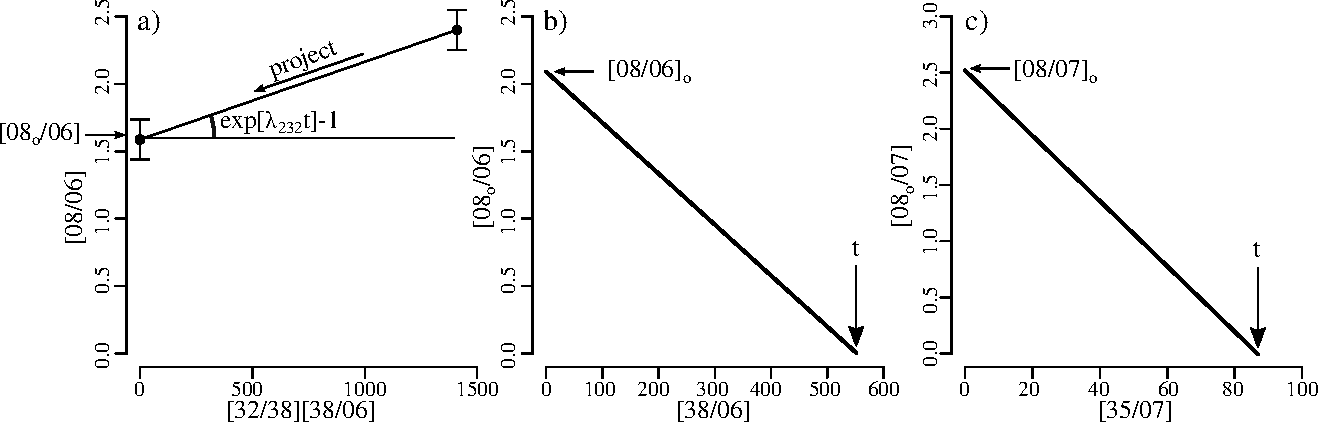
\includegraphics[width=\textwidth]{../figures/UPbisochron78.pdf}
    \captionof{figure}{The total-U-Th/Pb isochron is constructed in a
      similar way to the total-U/Pb isochron of
      Figure~\ref{fig:UPbisochron46}, but using the non-radiogenic
      \textsuperscript{208}Pb component instead of
      \textsuperscript{204}Pb. The first step in the calculation
      algorithm (panel a, left hand side of
      Equation~\ref{eq:total-U-Th/Pb-a}) is the removal of the
      radiogenic \textsuperscript{208}Pb component for each aliquot in
      the dataset. This is achieved by projecting the
      \textsuperscript{208}Pb/\textsuperscript{206}Pb ratio onto the
      \textsuperscript{208}Pb/\textsuperscript{206}Pb-axis along a
      line whose slope is given by the
      \textsuperscript{232}Th--\textsuperscript{208}Pb ingrowth
      equation. The algorithm then iterates over the parameters
      $[08/06]_\circ$, $[08/07]_\circ$ and $t$ until convergence is
      reached. Panel b) shows Equation~\ref{eq:total-U-Th/Pb-a},
      whereas panel c) shows Equation~\ref{eq:total-U-Th/Pb-b}.}
    \label{fig:UPbisochron78}
    \end{minipage}
    
\end{enumerate}

The parameterisation of these three discordia regression algorithms
implies that the discordance is caused by common Pb. However, the
results can also be used to interpret different scenarios such as
Pb-loss and mixing of different aged growth zones. These mechanisms
produce mixing lines between two concordant compositions on the
concordia line. These intercepts can be visualised using
\texttt{IsoplotR}'s Wetherill concordia function:

\noindent\begin{minipage}[t]{.5\linewidth}
\strut\vspace*{-\baselineskip}\newline
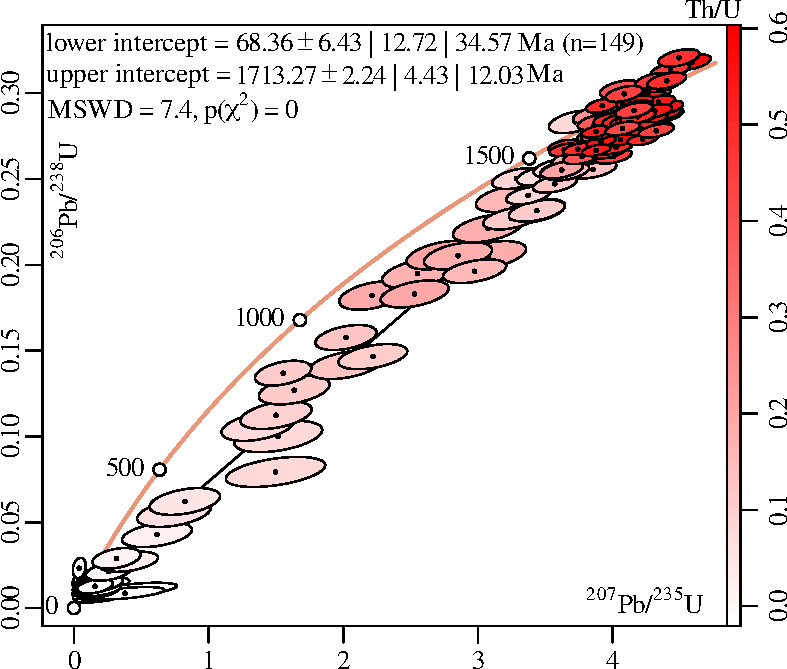
\includegraphics[width=\textwidth]{../figures/Hourigan.pdf}
\end{minipage}
\noindent\begin{minipage}[t]{.5\linewidth}
\captionof{figure}{Wetherill concordia diagram of a depth-drilling
  experiments for a cycle-by-cycle LA-ICP-MS depth drilling experiment
  by Jeremy Hourigan (UC Santa Cruz). As the laser drills through the
  grain, it exposes different mixtures between two compositional end
  members with distinct Th/U ratios as shown by the colour scale.
  \texttt{IsoplotR} fits the mixing line by semitotal-U/Pb regression
  (Equation~\ref{eq:semitotal-U/Pb}), the results are subsequently
  used to infer the upper intercept as well as the lower intercept
  with the concordia line.  }
\label{fig:Hourigan}
\end{minipage}

\section{Common Pb}
\label{sec:common-Pb}

There are a number of different strategies to remove the
non-radiogenic Pb component from U--(Th--)Pb measurements.  Which of
these is most appropriate depends on the data format and geological
setting:

\begin{enumerate}
\item In igneous and ortho-metamorphic rocks, where one can safely
  assume that all the aliquots are cogenetic and share the same common
  Pb composition, isochron regression is the most reliable method.
  \begin{enumerate}
  \item\label{it:isochroncommonpb} The common Pb composition as well
    as the concordia intercept age can be obtained using the methods
    reviewed in Section~\ref{sec:discordia}.\\
    
    \noindent\begin{minipage}[t]{\linewidth}
    \centering
    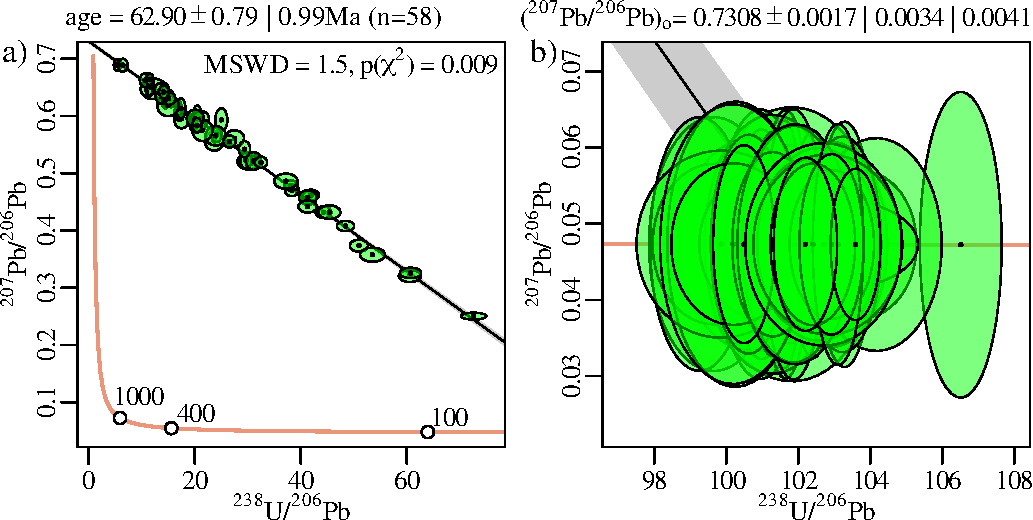
\includegraphics[width=.8\textwidth]{../figures/commonPbisochron13.pdf}
    \end{minipage}
    \begin{minipage}[t]{\linewidth}
      \centering
      \captionsetup{width=.8\textwidth}
      \captionof{figure}{
      For LA-ICP-MS data stored in formats 1--3, the isochron
      regression is done by semitotal-U/Pb regression (a). Projecting
      the data onto the concordia line (b) produces common-Pb
      corrected U--Pb compositions that are perfectly concordant by
      definition. The legend applies to both panels.}
    \label{fig:commonPbisochron13}
    \end{minipage}

    \noindent\begin{minipage}[t]{\linewidth}
    \centering
    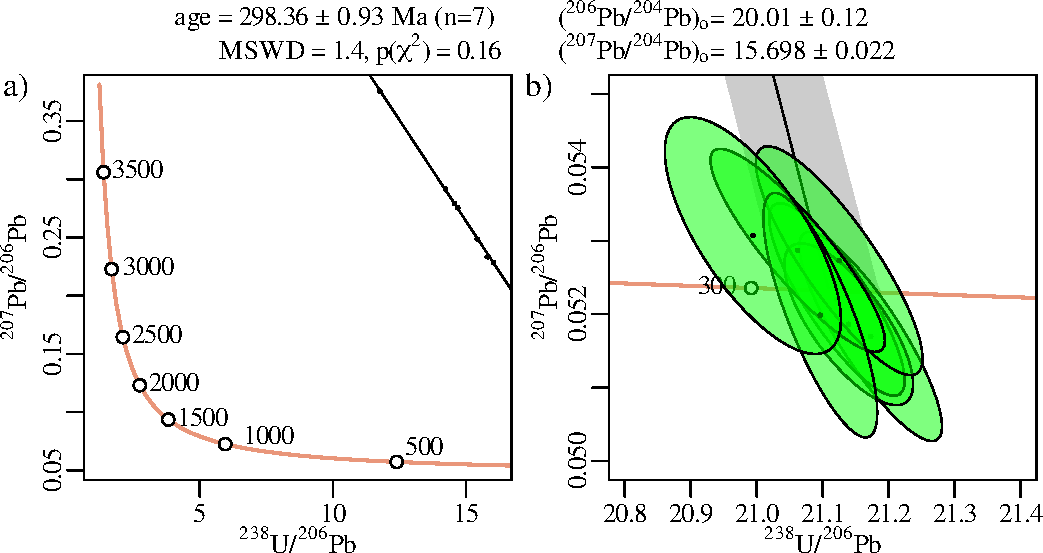
\includegraphics[width=.8\textwidth]{../figures/commonPbisochron46.pdf}
    \end{minipage}
    \begin{minipage}[t]{\linewidth}
      \centering \captionsetup{width=.8\textwidth} \captionof{figure}{
        For SIMS or TIMS data (note the small error ellipses) stored
        in formats 4--6, the isochron regression is done by total-U/Pb
        regression (a). Projecting the data along this 3-dimensional
        isochron line produces common-Pb corrected compositions that
        do not plot exactly on the concordia line. The legend applies
        to both panels.  }
    \label{fig:commonPbisochron46}
    \end{minipage}

  \item Alternatively, a nominal common Pb correction can be made by
    analysing a cogenetic mineral (such as feldspar) that is poor in
    U, and using its Pb composition as an `anchor' for a constrained
    discordia regression.\\

    \noindent\begin{minipage}[t]{\linewidth}
    \centering
    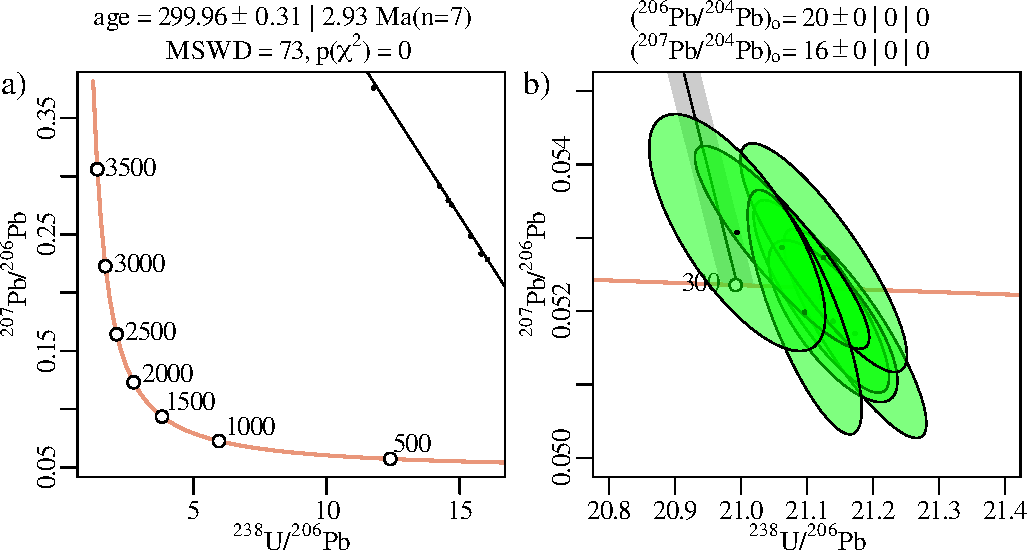
\includegraphics[width=.8\textwidth]{../figures/commonPbisochron46nominal.pdf}
    \end{minipage}
    \begin{minipage}[t]{\linewidth}
      \centering \captionsetup{width=.8\textwidth} \captionof{figure}{
        Common-Pb correction of the same data as
        Figure~\ref{fig:commonPbisochron13}, but using an isochron
        that is anchored at a nominal common Pb composition of
        \textsuperscript{206}Pb/\textsuperscript{204}Pb = 20 and
        \textsuperscript{207}Pb/\textsuperscript{204}Pb = 16 (note the
        zero uncertainties in the legend). In this example, this
        procedure is less accurate (intentionally, for the sake of
        illustration) than the unconstrained regression of
        Figure~\ref{fig:commonPbisochron13}.}
    \label{fig:commonPbisochron46}
    \end{minipage}
    
  \end{enumerate}
\item\label{it:separatecommonpb} In sedimentary and para-metamorphic
  rocks, in which the grains cannot safely be assumed to be cogenetic,
  each aliquot must be treated separately.
  \begin{enumerate}
  \item\label{it:nominalcommonpb} If there is some independent
    evidence to support a shared common-Pb composition for all the
    aliquots, then the radiogenic composition can be obtained by
    two-point isochron regression between that common-Pb composition
    and each aliquot.\\

    \noindent\begin{minipage}[t]{\linewidth}
    \centering
    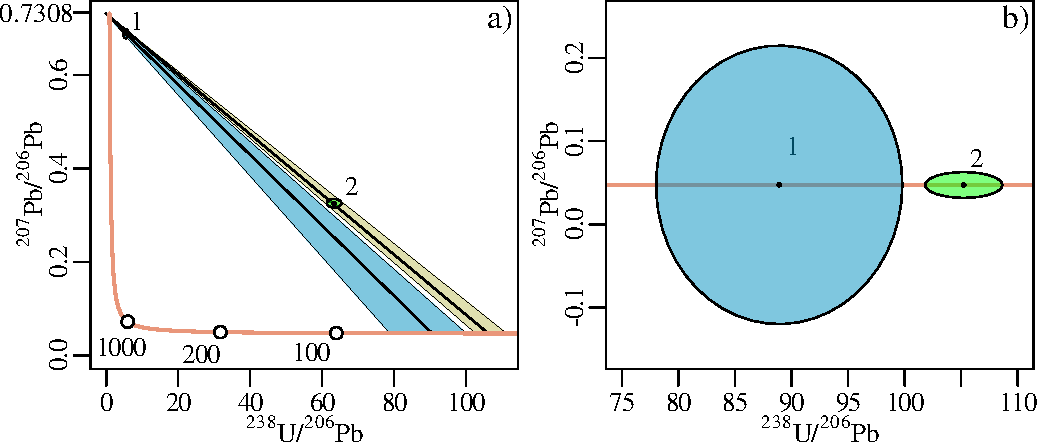
\includegraphics[width=.8\textwidth]{../figures/commonPbisochron13detrital.pdf}
    \end{minipage}
    \begin{minipage}[t]{\linewidth}
      \centering \captionsetup{width=.8\textwidth} \captionof{figure}{
        Common-Pb correction of two LA-ICP-MS based detrital
        measurements (formats 1--3) using the same nominal common Pb
        composition with
        \textsuperscript{206}Pb/\textsuperscript{206}Pb = 0.8.  Each
        aliquot forms its own mixing line, and its uncertainties are
        magnified by the extrapolation, in proportion to its distance
        to the concordia line. This is different from the joint
        isochron regression of Figures~\ref{fig:commonPbisochron13}
        and \ref{fig:commonPbisochron46}, in which all aliquots are
        projected parallel to a joint regression line and the
        uncertainties are only mildly affected by the extrapolation.}
    \label{fig:commonPbisochron13detrital}
    \end{minipage}
    
  \item\label{it:separate-stacey-kramers} In the absence of external
    evidence about the common Pb composition, one can infer the
    composition from the age using a mantle evolution model
    \citep[e.g.,][]{stacey1975}. If $t<3.7$~Ga:
    \begin{align}
      \left[\frac{{}^{206}Pb}{{}^{204}Pb}\right]_\circ = &
      11.152 + 9.74
      \left(\exp[\lambda_{238}3.7]-\exp[\lambda_{238}t]\right)
      \label{eq:stacey-kramers-a} \\
      \left[\frac{{}^{207}Pb}{{}^{204}Pb}\right]_\circ = &
      12.998 + 0.0707
      \left(\exp[\lambda_{235}3.7]-\exp[\lambda_{235}t]\right)
      \label{eq:stacey-kramers-b} \\
      \left[\frac{{}^{208}Pb}{{}^{204}Pb}\right]_\circ = &
      31.23 + 36.84
      \left(\exp[\lambda_{232}3.7]-\exp[\lambda_{232}t]\right)
      \label{eq:stacey-kramers-c}
    \end{align}

    Each value of $t$ represents a mixing line between a point on the
    concordia line and a point on the common-Pb intercept of the
    concordia diagram. Using the method of maximum likelihood,
    \texttt{IsoplotR} finds the mixing line that is closest to the
    each U--Pb measurement in a detrital dataset. For formats 1--3, it
    is generally possible to find an exact solution to this problem
    (i.e., the mixing line goes directly through the measurement).
    For formats 4--7, the problem is overconstrained and the fit is
    generally not perfect.

    \noindent\begin{minipage}[t][][b]{.4\linewidth}
    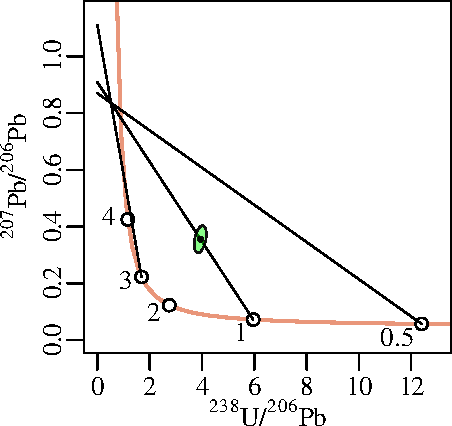
\includegraphics[width=\textwidth]{../figures/SK.pdf}
    \end{minipage}
    \begin{minipage}[t][][t]{.6\linewidth}
      \captionof{figure}{Three mixing lines between the radiogenic
        composition of 0.5, 1 and 3~Ga samples and the inferred
        Pb-composition of the mantle reservoir \citep[according
          to][]{stacey1975} from which these samples were
        hypothetically extracted. The y-intercepts correspond to
        \textsuperscript{207}Pb/\textsuperscript{206}Pb ratios of
        0.87, 0.91 and 1.11, respectively. For the error ellipse shown
        on this diagram, the mixing line at $t=1$~Ga best describes
        the composition of the sample. Hence, the common-Pb corrected
        age of this analysis is 1~Ga.  }
    \label{fig:commonPbSK}
    \end{minipage}
    
  \end{enumerate}
\end{enumerate}

\section{Initial disequilibrium}
\label{sec:U-Pb-disequilibrium}

Even though the U--Pb decay systems consist of numerous steps (14 for
\textsuperscript{238}U and 11 for \textsuperscript{235}U), this
complexity is ignored in conventional U--Pb geochronology and the
method is mathematically treated as a simple parent-daughter pair.
Section~\ref{sec:decay-series} showed that this assumption is
justified once a state of secular equilibrium is established between
all the intermediate daughter products in the decay chains.  Such
secular equilibrium automatically emerges after 1 to 2 million years.
Any disequilibrium that might exist prior to this can be used as a
chronometer in its own right, as discussed in
Section~\ref{ch:intro2Useries}.\\

Initial disequilibrium of the uranium decay series also affects the
accuracy of the U--Pb method. For example, ignoring any initial excess
\textsuperscript{234}U would result in an overestimated
\textsuperscript{206}Pb/\textsuperscript{238}U age, and any intial
\textsuperscript{231}Pa deficit would result in an underestimated
\textsuperscript{207}Pb/\textsuperscript{235}U age. Thus initial
disequilibrium is one mechanism to produce discordant results. The
effect of initial disequilibrium is relatively small in most
studies. It can be neglected in many geological applications, and is
is usually only a question of concern in high precision
geochronology.\\

However in U--Pb geochronology of young carbonates, the effect of
initial disequilibrium can be very significant, and may potentially
result in order-of-magnitude levels of bias. \texttt{IsoplotR} offers
three different strategies to deal with this bias:

\begin{enumerate}
\item If the intermediate daughter is sufficiently long lived, and the
  sample is sufficiently young to retain some of its disequilibrium,
  then the activity ratios can be back-calculated to the time of
  isotopic closure.  This strategy applies to
  \textsuperscript{234}U/\textsuperscript{238}U disequilibrium and,
  for very young samples, to
  \textsuperscript{230}Th/\textsuperscript{234}U disequilibrium.
\item For older samples and shorter lived intermediate daughters such
  as \textsuperscript{226}Ra ($t_{1/2}=1599$~yr), secular equilibrium
  has usually been re-established and the initial activity ratio must
  be assumed.
\item However in the case of
  \textsuperscript{230}Th/\textsuperscript{238}U disequilibrium in
  igneous rocks, the initial activity ratio can also be inferred from
  the \textsuperscript{232}Th/\textsuperscript{238}U ratio of the bulk
  host rocks. In this case we make the assumption that the bulk rock
  is representative for the starting material from which the datable
  mineral formed. Due to the chemical similarity between Th and Pa,
  the same procedure can be applied to
  \textsuperscript{231}Pa/\textsuperscript{238}U disequilibrium as
  well.
\end{enumerate}

\texttt{IsoplotR} solves the complex evolution of the decay series
using a matrix exponential approach developed by \citet{mclean2016}.
To illustrate the principles behind this approach, describe the
\textsuperscript{238}U--\textsuperscript{206}Pb decay chain in matrix
form:
\begin{equation}
  \frac{\partial}{\partial{t}}\left[
    \begin{array}{@{}c@{}}
      n38\\
      n34\\
      n30\\
      n26\\
      n06
    \end{array}
  \right]
  =
  \left[
    \begin{array}{cccccc}
      -\lambda_{38} & 0 & 0 & 0 & 0 & 0 \\
      \lambda_{38} & -\lambda_{34} & 0 & 0 & 0 & 0 \\
      0 & \lambda_{38} & -\lambda_{34} & 0 & 0 & 0 \\
      0 & 0 & \lambda_{34} & -\lambda_{30} & 0 & 0 \\
      0 & 0 & 0 & \lambda_{30} & -\lambda_{26} & 0 \\
      0 & 0 & 0 & 0 & \lambda_{26} & -\lambda_{26} \\
      0 & 0 & 0 & 0 & 0 & \lambda_{26}\\
    \end{array}
    \right]
  \left[
    \begin{array}{@{}c@{}}
      n38\\
      n34\\
      n30\\
      n26\\
      n06
    \end{array}
    \right]
  \label{eq:matrixdecay}
\end{equation}

\noindent where $n\ast\ast$ and $\lambda_{\ast\ast}$ stand for ``the
number of atoms and decay constant of nuclide $2\ast\ast$''.
Equation~\ref{eq:matrixdecay} is the matrix equivalent of the system
of equations that is represented in a simplified form by
Equations~\ref{eq:P1}--\ref{eq:D*}.  Just like the ordinary decay
equation is solved by an exponential function (Equation~\ref{eq:P2}),
so the matrix decay equation is solved by a matrix exponential:
\begin{equation}
  \left[
    \begin{array}{@{}c@{}}
      n38\\
      n34\\
      n30\\
      n26\\
      n06
    \end{array}
  \right]
  =
  \mbox{expm}\left(
  \left[
    \begin{array}{cccccc}
      -\lambda_{38} & 0 & 0 & 0 & 0 & 0 \\
      \lambda_{38} & -\lambda_{34} & 0 & 0 & 0 & 0 \\
      0 & \lambda_{38} & -\lambda_{34} & 0 & 0 & 0 \\
      0 & 0 & \lambda_{34} & -\lambda_{30} & 0 & 0 \\
      0 & 0 & 0 & \lambda_{30} & -\lambda_{26} & 0 \\
      0 & 0 & 0 & 0 & \lambda_{26} & -\lambda_{26} \\
      0 & 0 & 0 & 0 & 0 & \lambda_{26}\\
    \end{array}
    \right]
  t
  \right)
  \left[
    \begin{array}{@{}c@{}}
      n38\\
      n34\\
      n30\\
      n26\\
      n06
    \end{array}
    \right]_\circ
  \label{eq:matrixdecaysolution}
\end{equation}

\noindent which expresses the present day amounts as a function of the
initial amounts. Conversely, the equation can also be turned around to
express the initial amounts as a function of the present day amounts:
\begin{equation}
  \left[
    \begin{array}{@{}c@{}}
      n38\\
      n34\\
      n30\\
      n26\\
      n06
    \end{array}
  \right]_\circ
  =
  \mbox{expm}\left(
      -
  \left[
    \begin{array}{cccccc}
      -\lambda_{38} & 0 & 0 & 0 & 0 & 0 \\
      \lambda_{38} & -\lambda_{34} & 0 & 0 & 0 & 0 \\
      0 & \lambda_{38} & -\lambda_{34} & 0 & 0 & 0 \\
      0 & 0 & \lambda_{34} & -\lambda_{30} & 0 & 0 \\
      0 & 0 & 0 & \lambda_{30} & -\lambda_{26} & 0 \\
      0 & 0 & 0 & 0 & \lambda_{26} & -\lambda_{26} \\
      0 & 0 & 0 & 0 & 0 & \lambda_{26}\\
    \end{array}
    \right]
  t
  \right)
  \left[
    \begin{array}{@{}c@{}}
      n38\\
      n34\\
      n30\\
      n26\\
      n06
    \end{array}
    \right]
  \label{eq:matrixdecaysolutioninverse}
\end{equation}

The matrix exponential approach provides an elegant solution for all
three scenarios described above. Equation~\ref{eq:matrixdecaysolution}
can be used to construct a concordia diagram in the presence of
disequilibrium:\\

\noindent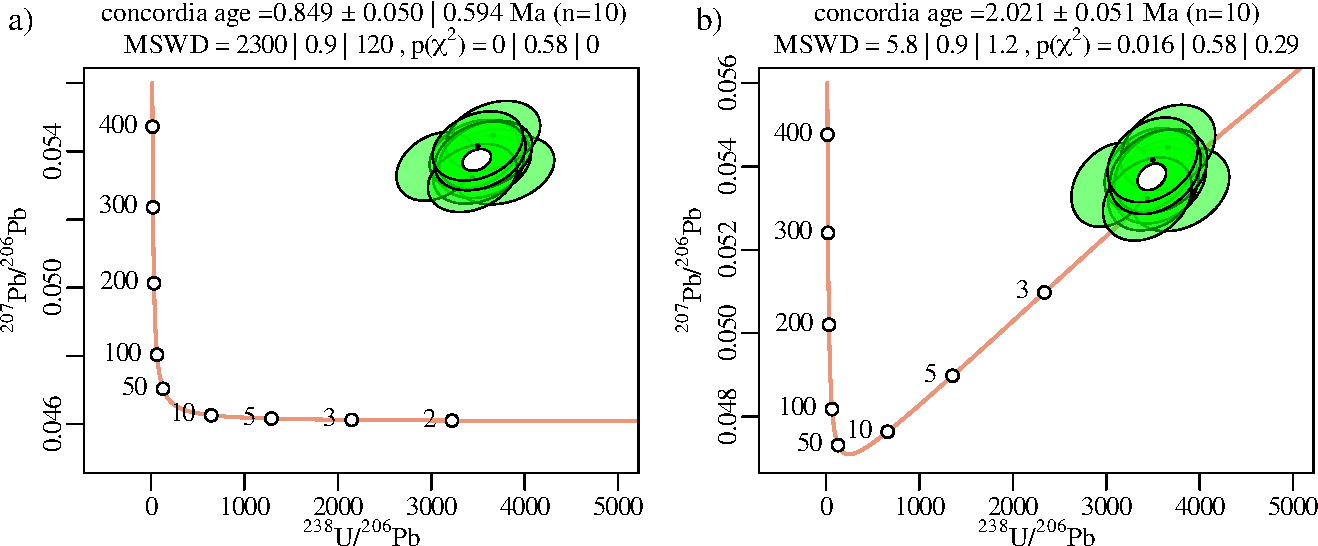
\includegraphics[width=\linewidth]{../figures/diseq.pdf}
\begingroup
\captionof{figure}{Tera-Wasserburg concordia diagram a) assuming
  secular equilibrium and b) accounting for secular disequilibrium with
  initial activity ratios of
  \textsuperscript{234}U/\textsuperscript{238}U = 0,
  \textsuperscript{230}Th/\textsuperscript{238}U = 2,
  \textsuperscript{226}Ra/\textsuperscript{238}U = 2 and
  \textsuperscript{231}Pa/\textsuperscript{235}U = 2.  These initial
  conditions cause the concordia line to curve upwards for young
  ages. Without the disequilibrium correction, the concordia age
  would be wrong by over 100\%.}
\label{fig:diseq}
\endgroup

\section{Discordance filters}
\label{sec:discfilter}

In detrital geochronology it is generally not possible to compute
multi-grain concordia ages and isochrons. In fact, each grain in a
detrital dataset has its own age and it is the entire distribution of
their values that carries scientific value. The question then arises
which method should be used to constrain the age distribution.
\texttt{IsoplotR} offers a number of options:

\begin{enumerate}
\item use the \textsuperscript{206}Pb/\textsuperscript{238}U date
  ($t_{68}$).
\item use the \textsuperscript{207}Pb/\textsuperscript{235}U date
  ($t_{75}$).  Given that the half-life of \textsuperscript{235}U is
  more than six times shorter than that of \textsuperscript{238}U, and
  that \textsuperscript{235}U is more than 100 times less abundant
  than \textsuperscript{238}U, little \textsuperscript{207}Pb has been
  produced during the last billion years of Earth history compared to
  \textsuperscript{206}Pb. Consequently, the
  \textsuperscript{207}Pb/\textsuperscript{235}U method is less
  precise than the \textsuperscript{206}Pb/\textsuperscript{238}U
  method during the Phanerozoic and Neoproterozoic, but more precise
  prior to that.
\item use the \textsuperscript{207}Pb/\textsuperscript{206}Pb date
  ($t_{76}$).  Like the
  \textsuperscript{207}Pb/\textsuperscript{235}U, also the
  \textsuperscript{207}Pb/\textsuperscript{206}Pb method is more
  precise than the \textsuperscript{206}Pb/\textsuperscript{238}U
  method for old grains, and less precise for young ones.  The gradual
  shift in sensitivity between the
  \textsuperscript{206}Pb/\textsuperscript{238}U and
  \textsuperscript{207}Pb/\textsuperscript{206}Pb methods is visible
  in the slope of a Tera-Wasserburg concordia line, which is steep at
  old ages (high \textsuperscript{207}Pb/\textsuperscript{206}Pb
  gradient w.r.t. time) and shallow at young ages (low
  \textsuperscript{238}U/\textsuperscript{206}Pb gradient
  w.r.t. time).
\item switch from \textsuperscript{206}Pb/\textsuperscript{238}U to
  \textsuperscript{207}Pb/\textsuperscript{206}Pb at some point during
  the Proterozoic. This ensures good precision for all grains but
  introduces two practical issues. First, it requires the selection of
  a discrete discordance cutoff between the two methods.  Second, the
  sudden switch between the
  \textsuperscript{206}Pb/\textsuperscript{238}U and
  \textsuperscript{207}Pb/\textsuperscript{206}Pb clocks may be marked
  by a discrete step in the age spectrum. This step is entirely
  artificial and obscures any geologically significant events that
  might occur around the same time.
\item use the single grain concordia date ($t_c$), which is calculated
  by applying Equation~\ref{eq:concordiaAgeWetherill} or
  \ref{eq:concordiaAgeTW} separately to each grain. This approach
  avoids the need to switch between different methods, and offers
  superior precision to any of the other methods across the entire
  geologic time scale.
\end{enumerate}

Once a chronometer has been chosen, it is advisable to `filter' the
data before plotting them as a KDE or CAD, so as to remove the most
discordant analyses. It may be so that the common Pb correction of
Section~\ref{sec:common-Pb} removes much (or all, in the case of
formats 1--3) discordance. But accuracy of single-grain common Pb
corrections decreases quickly with increasing distance from the
concordia line. For example, in
Figure~\ref{fig:commonPbisochron13detrital}, aliquot~1 should probably
not be used to constrain the age distribution. \texttt{IsoplotR}
offers six different definitions of discordance that can be used to
filter U--Pb data:

\begin{enumerate}
  \item The relative age discordance:
    \begin{equation}
      d_{r} = 1 - t_{68}/t_{76}
      \label{eq:dr}
    \end{equation}
    This is the most widely used criterion today.  It is more likely
    to remove young grains than old ones, and strongly skews the age
    distribution towards old age components as a result.
  \item The absolute age discordance:
    \begin{equation}
      d_{t} = t_{76} - t_{68}
      \label{eq:dt}
    \end{equation}
    This definition is not very widely used. But it illustrates the
    dramatic effect that the discordance definition can have on the
    filtered age distibutions. Compared with the relative age filter,
    it is more likely to reject old grains, and less likely to reject
    young ones. It even allows physically impossible negative
    \textsuperscript{207}Pb/\textsuperscript{206}Pb ages to pass
    through it.
  \item The p-value based discordance filter:
    \begin{equation}
      d_p = \mbox{Prob}\left(s > S_c | S_c \sim \chi^2_2\right)
      \label{eq:dp}
    \end{equation}
    \noindent where $S_c$ is defined in
    Equation~\ref{eq:concordiaAgeWetherill}/\ref{eq:concordiaAgeTW}.
    $d_p$ may have intuitive appeal as an `objective' definition. But
    it has an undesirable negative effect on the precision and
    accuracy of the filtered results.  This is because the p-value
    definition affects grains differently depending on their
    analytical precision.\\

    For example, consider a 1.5~Ga zircon that is $d_r=1\%$
    discordant. If this grain were analysed by LA-ICP-MS with an
    analytical precision of 2\%, say, then it would pass the
    chi-square test and be accepted as being concordant. However, if
    that same grain were analysed by TIMS with a precision of 0.2\%,
    then the p-value criterion would reject it as being discordant. It
    seems fundamentally wrong that an imprecise analytical method
    would be favoured over a precise one. This is a pertinent problem
    because technical innovations are increasing the precision of all
    analytical approaches to U--Pb geochronology.  As precision
    improves, so does the ability to detect ever small degrees of
    discordance. Using the p-value criterion, there may come a time
    when no zircon passes this filter.  Hence it is best not to use
    this filter, but \texttt{IsoplotR} offers it nonetheless for the
    sake of completeness and to allow reproducing published results.
  \item The Stacey-Kramers discordance filter
    \begin{equation}
      d_{sk} = 1 - r_{86}/r_{86}^\ast
    \end{equation}
    \noindent where $r_{86}$ and $r_{86}^\ast$ are the
    \textsuperscript{238}U/\textsuperscript{206}Pb ratios before and
    after common Pb correction, assumes that discordance is solely
    caused by common Pb contamination. If this assumption is correct,
    then the $d_{sk}$ filter will produce the most accurate age
    distributions, provided that a \citet{stacey1975} common Pb
    correction is applied to the filtered data afterwards.
  \item The perpendicular Aitchison distance
    \begin{equation}
      d_{a} = dx(t_{68}) \sin\!\left(\arctan\!\left[
        \frac{dy(t_{76})}{dx(t_{68})} \right] \right)
    \end{equation}
    \noindent represents the logarithmic distance from the measurement
    to the concordia line in log-log space
    \citep{vermeesch2021}. $dx(\ast)$ and $dy(\ast)$ are the
    horizontal and vertical component of this distance. $d_a$ produces
    a parallel acceptance zone around the (log-transformed) concordia
    line. This filter is most likely to reject `middle aged' zircon
    grains, between 1000 and 2000~Ma, where the age resolving power of
    the U--Pb method is greatest. Above and below this interval, the
    $d_a$ criterion is more forgiving. This behaviour is desirable
    because natural samples tend to exhibit more age discordance below
    1000~Ma and above 2000~Ma than between these dates.

    \noindent\begin{minipage}[t][][b]{.45\linewidth}
    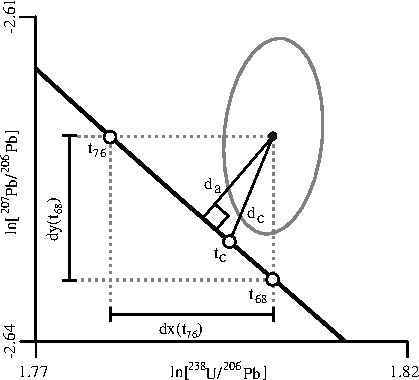
\includegraphics[width=\textwidth]{../figures/Aitchison.pdf}
    \end{minipage}
    \begin{minipage}[t][][t]{.55\linewidth}
      \captionof{figure}{Illustration of the two logratio distance
        definitions of discordance. $d_a$ is the perpendicular
        Aitchison distance from the measured logratio to the concordia
        line. $d_c$ is the Aitchison distance measured along a line
        connecting the measured value and the concordia composition.}
    \label{fig:da}
    \end{minipage}
    
  \item The concordia distance
    \begin{equation}
    d_c = \mbox{sgn}[t_{76}-t_{68}] \sqrt{ dx(t_c)^2 + dy(t_c)^2 }
    \end{equation}
    is a modified version of the $d_a$ criterion that takes into
    account the uncertainties of the U--Pb isotopic composition. It
    represents the distance (in log-log space) from the measurement to
    the U--Pb composition of the concordia age.  Its effects on the
    U--Pb age distributions are more difficult to visualise but are
    similar to those of the $d_a$ criterion. Empirical evidence
    suggests that this filter is optimal in the sense that it has a
    minimal effect on the shape of the age distribution: it results in
    a tightening of subpopulations without changing their position or
    relative size \citep{vermeesch2020}.
\end{enumerate}

\noindent\begin{minipage}[t][][b]{.45\linewidth}
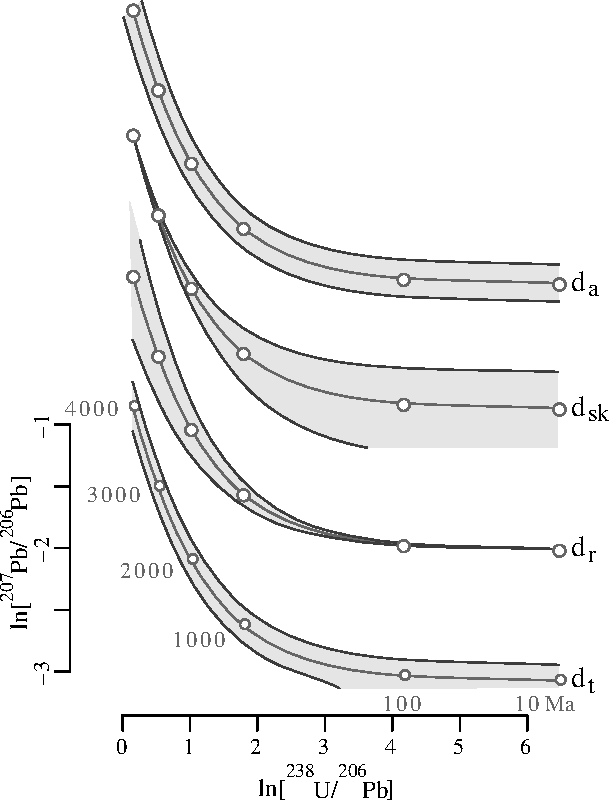
\includegraphics[width=\textwidth]{../figures/TW-option-1234.pdf}
\end{minipage}
\begin{minipage}[t][][t]{.55\linewidth}
  \captionof{figure}{ Discordance cutoffs for four of the six
    discordance definitions. The $d_{p}$ and $d_c$ criteria are not
    shown because they depend on the analytical uncertainty of the
    measurements, which may vary between studies. The grey envelopes
    mark cutoff values of $d_r=20\%$ (relative age filter),
    $d_t=300$~Ma (absolute age filter), $d_{sk}=2\%$ (Stacey--Kramers
    filter) and $d_{a}=15\%$ (perpendicular Aitchison distance) on a
    Tera-Wasserburg concordia diagram, which is plotted in logarithmic
    space to provide a more balanced view of the old and young ends of
    the time scale. The $d_{sk}$ and $d_t$ envelopes are truncated
    where they cross over into physically impossible negative isotope
    ratio space.}
  \label{fig:agediscordance}
\end{minipage}

\printbibliography[heading=subbibliography]

\end{refsection}
